\ifx\wholebook\relax \else
% ------------------------ 

\documentclass{article}
%------------------- Other types of document example ------------------------
%
%\documentclass[twocolumn]{IEEEtran-new}
%\documentclass[12pt,twoside,draft]{IEEEtran}
%\documentstyle[9pt,twocolumn,technote,twoside]{IEEEtran}
%
%-----------------------------------------------------------------------------
%%
% loading packages
%
\newif\ifpdf
\ifx\pdfoutput\undefined % We're not running pdftex
  \pdffalse
\else
  \pdftrue
\fi
%
%
\ifpdf
  \RequirePackage[pdftex,%
            CJKbookmarks,%
       bookmarksnumbered,%
              colorlinks,%
          linkcolor=blue,%
              hyperindex,%
        plainpages=false,%
       pdfstartview=FitH]{hyperref}
\else
  \RequirePackage[dvipdfm,%
             CJKbookmarks,%
        bookmarksnumbered,%
               colorlinks,%
           linkcolor=blue,%
               hyperindex,%
         plainpages=false,%
        pdfstartview=FitH]{hyperref}
  \AtBeginDvi{\special{pdf:tounicode GBK-EUC-UCS2}} % GBK -> Unicode
\fi
\usepackage{hyperref}

% other packages
%-----------------------------------------------------------------------------
\usepackage{graphicx, color}
\usepackage{CJK}
%
% for programming 
%
\usepackage{verbatim}
\usepackage{listings}


\lstdefinelanguage{Smalltalk}{
  morekeywords={self,super,true,false,nil,thisContext}, % This is overkill
  morestring=[d]',
  morecomment=[s]{"}{"},
  alsoletter={\#:},
  escapechar={!},
  literate=
    {BANG}{!}1
    {UNDERSCORE}{\_}1
    {\\st}{Smalltalk}9 % convenience -- in case \st occurs in code
    % {'}{{\textquotesingle}}1 % replaced by upquote=true in \lstset
    {_}{{$\leftarrow$}}1
    {>>>}{{\sep}}1
    {^}{{$\uparrow$}}1
    {~}{{$\sim$}}1
    {-}{{\sf -\hspace{-0.13em}-}}1  % the goal is to make - the same width as +
    %{+}{\raisebox{0.08ex}{+}}1		% and to raise + off the baseline to match -
    {-->}{{\quad$\longrightarrow$\quad}}3
	, % Don't forget the comma at the end!
  tabsize=2
}[keywords,comments,strings]

\lstloadlanguages{C++, Lisp, Haskell, Python, Smalltalk}

% ======================================================================

\def\BibTeX{{\rm B\kern-.05em{\sc i\kern-.025em b}\kern-.08em
    T\kern-.1667em\lower.7ex\hbox{E}\kern-.125emX}}

\newtheorem{theorem}{Theorem}

%
% mathematics
%
\newcommand{\be}{\begin{equation}}
\newcommand{\ee}{\end{equation}}
\newcommand{\bmat}[1]{\left( \begin{array}{#1} }
\newcommand{\emat}{\end{array} \right) }
\newcommand{\VEC}[1]{\mbox{\boldmath $#1$}}

% numbered equation array
\newcommand{\bea}{\begin{eqnarray}}
\newcommand{\eea}{\end{eqnarray}}

% equation array not numbered
\newcommand{\bean}{\begin{eqnarray*}}
\newcommand{\eean}{\end{eqnarray*}}

\RequirePackage{CJK,CJKnumb,CJKulem,CJKpunct}
% we use CJK as default environment
\AtBeginDocument{\begin{CJK*}{GBK}{song}\CJKtilde\CJKindent\CJKcaption{GB}}
\AtEndDocument{\clearpage\end{CJK*}}

%
% loading packages
%

\RequirePackage{ifpdf}

%
%
\ifpdf
  \RequirePackage[pdftex,%
       bookmarksnumbered,%
              colorlinks,%
          linkcolor=blue,%
              hyperindex,%
        plainpages=false,%
       pdfstartview=FitH]{hyperref}
\else
  \RequirePackage[dvipdfm,%
        bookmarksnumbered,%
               colorlinks,%
           linkcolor=blue,%
               hyperindex,%
         plainpages=false,%
        pdfstartview=FitH]{hyperref}
\fi
\usepackage{hyperref}

% other packages
%--------------------------------------------------------------------------
\usepackage{graphicx, color}
\usepackage{subfig}

\usepackage{amsmath, amsthm, amssymb} % for math
\usepackage{exercise} % for exercise

%
% for programming 
%
\usepackage{verbatim}
\usepackage{listings}
%\usepackage{algorithmic} %old version; we can use algorithmicx instead
\usepackage{algorithm} 
\usepackage[noend]{algpseudocode} %for pseudo code, include algorithmicsx automatically
\usepackage{makeidx} % for index support


\lstdefinelanguage{Smalltalk}{
  morekeywords={self,super,true,false,nil,thisContext}, % This is overkill
  morestring=[d]',
  morecomment=[s]{"}{"},
  alsoletter={\#:},
  escapechar={!},
  literate=
    {BANG}{!}1
    {UNDERSCORE}{\_}1
    {\\st}{Smalltalk}9 % convenience -- in case \st occurs in code
    % {'}{{\textquotesingle}}1 % replaced by upquote=true in \lstset
    {_}{{$\leftarrow$}}1
    {>>>}{{\sep}}1
    {^}{{$\uparrow$}}1
    {~}{{$\sim$}}1
    {-}{{\sf -\hspace{-0.13em}-}}1  % the goal is to make - the same width as +
    %{+}{\raisebox{0.08ex}{+}}1		% and to raise + off the baseline to match -
    {-->}{{\quad$\longrightarrow$\quad}}3
	, % Don't forget the comma at the end!
  tabsize=2
}[keywords,comments,strings]

\lstloadlanguages{C++, Lisp, Haskell, Python, Smalltalk}

% ======================================================================

\def\BibTeX{{\rm B\kern-.05em{\sc i\kern-.025em b}\kern-.08em
    T\kern-.1667em\lower.7ex\hbox{E}\kern-.125emX}}

%
% mathematics
%
\newcommand{\be}{\begin{equation}}
\newcommand{\ee}{\end{equation}}
\newcommand{\bmat}[1]{\left( \begin{array}{#1} }
\newcommand{\emat}{\end{array} \right) }
\newcommand{\VEC}[1]{\mbox{\boldmath $#1$}}

% numbered equation array
\newcommand{\bea}{\begin{eqnarray}}
\newcommand{\eea}{\end{eqnarray}}

% equation array not numbered
\newcommand{\bean}{\begin{eqnarray*}}
\newcommand{\eean}{\end{eqnarray*}}

\newtheorem{theorem}{Theorem}[section]
\newtheorem{lemma}[theorem]{Lemma}
\newtheorem{proposition}[theorem]{Proposition}
\newtheorem{corollary}[theorem]{Corollary}


\setcounter{page}{1}

\begin{document}

\fi
%--------------------------

% ================================================================
%                 COVER PAGE
% ================================================================

\title{Divide and conquer, Quick sort V.S. Merge sort}

\author{Liu~Xinyu
\thanks{{\bfseries Liu Xinyu } \newline
  Email: liuxinyu95@gmail.com \newline}
  }

\markboth{Quick sort V.S. Merge sort}{AlgoXY}

\maketitle

\ifx\wholebook\relax
\chapter{Divide and conquer, Quick sort V.S. Merge sort}
\numberwithin{Exercise}{chapter}
\fi

% ================================================================
%                 Introduction
% ================================================================
\section{Introduction}
\label{introduction} 

It's proved that the best approximate performance of comparison based sorting is $O(N \lg N)$ \cite{TAOCP}.
In this chapter, two divide and conquer sorting algorithms are introduced. Both of them
perform in $O(N \lg N)$ time. One is quick sort. It is
the most popular sorting algorithm. Quick sort has been well studied, many programming libraries provide
sorting tool based on quick sort. 

In this chapter, we'll first introduce the idea of of quick sort, which demonstrates the power of divide 
and conquer strategy well. Several variants will be explained, and we'll see when quick sort performs poor
in some special cases. That the algorithm is not able to partition the sequence in balance.

In order to solve the unbalanced partition problem, we'll next introduce about merge sort, which ensure
the sequence to be well partitioned in all the cases. Some variants of merge sort, including nature merge
sort, bottom-up merge sort are shown as well.

Similar as other chapters, all the algorithm will be realized in both imperative and functional approaches.

% ================================================================
% Quick sort
% ================================================================
\section{Quick sort}
\index{Quick sort}

Consider a teacher arranges a group of kids in kindergarten to stand in a line for some game.
The kids need stand in order of their heights, that the shortest one stands on the left most,
while the tallest stands on the right most. How can the teacher instruct these kids, so that
they can stand in a line by themselves?

\begin{figure}[htbp]
 \centering
 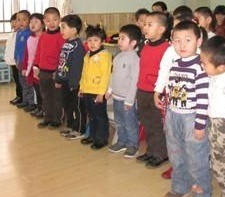
\includegraphics[scale=0.8]{img/kids-inline.eps}
 \caption{Instruct kids to stand in a line}
 \label{fig:knuth-ssort}
\end{figure}

There are many strategy, and the quick sort approach can be applied here:

\begin{enumerate}
  \item The first kid raises his/her hand. The kids who are shorter than him/her stands to the left to this child; the kids who are taller than him/her stands to the right of this child;
  \item All the kids move to the left if there are repeat the above step; all the kids move to the right repeat the same step as well.
\end{enumerate}

Suppose a group of kids with their heights as $\{102, 100, 98, 95, 96, 99, 101, 97\}$ with [cm] as the unit. 
The following table illustrate how they stand in order of height by folllowing this method.

\begin{tabular}{ | c c c c c c c c |}
\hline
{\bf 102} & 100 & 98 & 95 & 96 & 99 & 101 & 97 \\
{\bf 100} & 98 & 95 & 96 & 99 & 101 & 97 & {\em 102} \\
{\bf 98} & 95 & 96 & 99 & 97 & {\em 100} & 101 & {\em 102} \\
{\bf 95} & 96 & 97 & {\em 98} & 99 & {\em 100} & {\em 101} & {\em 102} \\
{\em 95} & {\bf 96} & 97 & {\em 98} & {\em 99} & {\em 100} & {\em 101} & {\em 102} \\
{\em 95} & {\em 96} & 97 & {\em 98} & {\em 99} & {\em 100} & {\em 101} & {\em 102} \\
{\em 95} & {\em 96} & {\em 97} & {\em 98} & {\em 99} & {\em 100} & {\em 101} & {\em 102} \\
\hline
\end{tabular}

At the beginning, the first child with height 102 cm raises his/her hand. We call this kid the pivot and mark
his height in bold.
It happens that this is the tallest kid.
So all others stands to the left side, which is represented in the second row of above table. Note that
the child with height 102 cm is in the final ordered position, thus we mark it italic. Next the kid with
height 100 cm raise hand, so the children of heights 98, 95, 96 and 99 cm stand to his/her left, and there
is only 1 child of height 101 cm who is taller than this pivot kid. So he stands to the right hand.
The 3rd row in the table shows this stage accordingly. After that, the child of 98 cm high is seleced
as pivot on left hand; while the child of 101 cm high on the right is selected as pivot. Since there
are no other kids in the unsorted group with 101 cm as pivot, this small group is ordered already and
the kid of height 101 cm is in the final proper postion. The same method is applied to the group of kids
which haven't been in correct order until all of them are stands in the final position.

\subsection{Basic version}
Summarize the above insruction leads to the recursive description of quick sort. In order to sort a sequence
of elements $L$.

\begin{itemize}
\item If $L$ is empty, the result is obviously empty; This is the trivial edge case;
\item Otherwise, select an arbitrary element in $L$ as a pivot, recursively sort all elements not greater than $L$, put
the result on the left hand of the pivot, {\em and} recursively sort all elements which are greater than $L$, put
the result on the right hand of the pivot.
\end{itemize}

Note that the emphasized word {\em and}, we don't use `then' here, which indicate it's quite OK that 
the recursive sort on the left and right can be done in parrallel. We'll return this parallism topic soon.

Quick sort was first developed by C. A. R. Hoare in 1960 \cite{TAOCP}, \cite{wiki-qs}. What we describe here
is a basic version. Note that it doesn't state how to select the pivot. We'll see soon that the pivot selection
affects the performance of quick sort later.

The most simple method to select the pivot is always choose the first one so that quick sort can be formalized 
as the following.

\be
sort(L) = \left \{
  \begin{array}
  {r@{\quad:\quad}l}
  \Phi & L = \Phi \\
  sort(\{ x | x \in L', x \leq l_1 \} \cup \{ l_1 \} \cup sort(\{ x | x \in L', l_1 < x \}) & otherwise \\
  \end{array}
\right.  
\ee

Where $l_1$ is the first element of the non-empty list $L$, and $L'$ contains the rest elements $\{l_2, l_3, ...\}$.
Note that we use Zermelo Frankel expression (ZF expresssion for short), which is also known as list
comprehension. A ZF expression $\{ a | a \in S, p_1(a), p_2(a), ... \}$ means take all element in set $S$,
if it satisfies the predication $p_1, p_2, ...$. The result is also a list. Please refer to the appendix
about list in this book for detail.

It's quite straightforward to translate this equation to real code if list comprehension is supported.
The following Haskell code is give for example:

\lstset{language=Haskell}
\begin{lstlisting}
sort [] = []
sort (x:xs) = sort [y | y<-xs, y <= x] ++ [x] ++ sort [y | y<-xs, x < y]
\end{lstlisting}

This might be the shortest quick sort program in the world at the time when this book is written. Even
a verbose version is still very expressive:

\lstset{language=Haskell}
\begin{lstlisting}
sort [] = []
sort (x:xs) = as ++ [x] ++ bs where
    as = sort [ a | a <- xs, a <= x]
    bs = sort [ b | b <- xs, x < b]
\end{lstlisting}

There are some variants of this basic quick sort program, such as using explicit filtering instead of
list comprehension. The following Python program demonstrates this for example:

\lstset{language=Python}
\begin{lstlisting}
def sort(xs):
    if xs == []:
        return []
    pivot = xs[0]
    as = sort(filter(lambda x : x <= pivot, xs[1:]))
    bs = sort(filter(lambda x : pivot < x, xs[1:]))
    return as + [pivot] + bs
\end{lstlisting}

\subsection{Strict weak ordering}
We assume the elements are sorted in monotonic none decreasing order so far. It's quite possible to customize
the algorithm, so that it can sort the elements in other ordering criteria. This is necessary in practice because
users may sort numbers, strings, or other complex objects (even list of lists for example) and so on.

The typical generic solution is to abstract the comparison as a parameter as we mentioned in chapters about 
insertion sort and selection sort. Although it needn't the total ordering, the comparison must satisfy 
{\em strict weak ordering} at least \cite{wiki-total-order} \cite{wiki-sweak-order}.

For the sake of brevity, we only considering sort the elements by using less than or equal 
(equivelent to not greater than) in the rest of the chapter.

\subsection{Partition}
\index{Quick sort!partition}
Observing that the basic version actually takes two passes to find all elements not greater than the pivot and 
the rest. Such partition can be accomplished by only one pass. We explicitly define the partition as below.

\be
partition(p, L) = \left \{
  \begin{array}
  {r@{\quad:\quad}l}
  (\Phi, \Phi) & L = \Phi \\
  (\{ l_1 \} \cup A, B) & p(l_1), (A, B) = partition(p, L') \\
  (A, \{ l_1 \} \cup B) & \lnot p(l_1)
  \end{array}
\right.  
\ee

The quick sort can be modified accordingly.

\be
sort(L) = \left \{
  \begin{array}
  {r@{\quad:\quad}l}
  \Phi & L = \Phi \\
  sort(A) \cup \{l_1\} \cup sort(B) & otherwise, (A, B) = partition(\lambda_x x \leq l_1, L')
  \end{array}
\right.  
\ee

Translating this new algorithm into Haskell yields the below code.

\lstset{language=Haskell}
\begin{lstlisting}
sort [] = []
sort (x:xs) = sort as ++ [x] ++ sort bs where
    (as, bs) = partition (<= x) xs

partition _ [] = ([], [])
partition p (x:xs) = let (as, bs) = partition p xs in
    if p x then (x:as, bs) else (as, x:bs)
\end{lstlisting}

The concept of parition is very cirtical to quick sort. Partition is also very important to many
other sort algorithms. We'll explain how it generally affects the sorting methodology by the end
of this chapter. Before further discussion about fine tuning of quick sort specific partition, let's
see how to realize it in-place imperatively.

There many partition methods. The one given by Nico Lomuto \cite{pearls} \cite{CLRS} will be used here as it's
easy to understand. We'll show other partition algorithm soon and see how it affects the performance.

TODO: imperative partition and in place quick sort

TODO: 
partition by folding
Accumulated partition
Accumulated FP version

\begin{Exercise}
\begin{itemize}
\item Implement the recursive basic quick sort algorithm in your favorite imperative programming language.
\end{itemize}  
\end{Exercise}

\section{Performance analysis for quick sort}

Minor problem:
  Duplicated elements

Major problem:
  Worst case

% ================================================================
% Minor Improvement for quick sort
% ================================================================

\section{Engineering Improvement}

\subsection{Engineering soltuion to duplicted elements}
TODO: improved partition (refer to Jon Bentley)

TODO: Tenery quick sort

\section{Engineering solution to worst case}
TODO: 3 median

\section{Other engineering practice}
TODO: Revert to insertion sort: Sedgewick's 

\section{Side words}
TODO: Relationship between quick sort and tree sort (deforestration, Richard Bird)

% ================================================================
% Improvement 2
% ================================================================

\section{Major improvement}


\section{Short summary} 
From easy/hard partition, easy/hard merge point of view

TODO:

\begin{thebibliography}{99}

\bibitem{TAOCP}
Donald E. Knuth. ``The Art of Computer Programming, Volume 3: Sorting and Searching (2nd Edition)''. Addison-Wesley Professional; 2 edition (May 4, 1998) ISBN-10: 0201896850 ISBN-13: 978-0201896855

\bibitem{CLRS}
Thomas H. Cormen, Charles E. Leiserson, Ronald L. Rivest and Clifford Stein. 
``Introduction to Algorithms, Second Edition''. ISBN:0262032937. The MIT Press. 2001

\bibitem{pearls}
Jon Bentley. ``Programming pearls, Second Edtion''. Addison-Wesley Professional; 1999. ISBN-13: 978-0201657883

\bibitem{wiki-qs}
Wikipedia. ``Quicksort''. http://en.wikipedia.org/wiki/Quicksort

\bibitem{wiki-sweak-order}
Wikipedia. ``Strict weak order''. http://en.wikipedia.org/wiki/Strict\_weak\_order

\bibitem{wiki-total-order}
Wikipedia. ``Total order''. http://en.wokipedia.org/wiki/Total\_order

\end{thebibliography}

\ifx\wholebook\relax\else
\end{document}
\fi
